% Ausarbeitung SAJ 
% FH Augsburg 
%
%
%
%
\documentclass[titlepage, 12pt,a4paper]{scrartcl}
%scrartcl
\usepackage[ngerman]{babel}
%\usepackage[latin1]{inputenc}
\usepackage[T1]{fontenc}
\usepackage{ucs}            % Eventuell benötigt
\usepackage[utf8x]{inputenc}

\usepackage{setspace}           % Paket fuer den Zeilenabstand
\onehalfspacing                 % Setzt den Zeilenabstand auf 1.5

\usepackage{graphicx}
\usepackage{listings}
\usepackage[hyphens]{url}
%\usepackage{breakurl}
\usepackage{hyperref}
\usepackage[usenames]{color}
\definecolor{light-gray}{gray}{0.90}
\usepackage[fixlanguage]{babelbib}
\usepackage{listings}
%\lstset{numbers=left, numberstyle=\tiny, numbersep=5pt}
%\lstset{language=Perl}
\lstloadlanguages{bash,XML,HTML, PHP, Python}
\selectbiblanguage{german}
\usepackage{makeidx}
%\usepackage{pifont}
\makeindex
%\usepackage{fancyhdr}
%\setlength{\headheight}{15.2pt}
%\pagestyle{fancy}


\author{Moritz Schächterle, Dominik Heimstädt \& Andrés Cuartas}
\title{- Studienarbeit Python - \\ WM-Tippspiel 2010 \\}
%\date{11-Dez-2007}

\pagestyle{myheadings}
\markright{Schaechterle, Heimstaedt \& Cuartas}
\lstset{
	inputencoding=utf8x,
	extendedchars=\true,
	language=Python,
	basicstyle=\tiny,
	keywordstyle=\bfseries\color{green},
	identifierstyle=,
	%commentstyle=\color{gray},	
	%stringstyle=\itshape\color{darkred},
	numbers=left,
	numberstyle=\tiny,
	stepnumber=1,
	breaklines=true,
	frame=none,
	showstringspaces=false,
	tabsize=4,
	backgroundcolor=\color{light-gray},
	captionpos=b,
	float=htbp,
	frameround=fttt
}


%\lstset{language=XML, stringstyle=\ttfamily, tabsize=2, basicstyle=\small, breaklines=true, backgroundcolor=\color{light-gray}, frameround=fttt}
%              
% WORKAROUND, damit lstlistoflistings funktioniert: 
% Quelle: http://www.komascript.de/node/477
%
\makeatletter% --> De-TeX-FAQ
\renewcommand*{\lstlistoflistings}{%
  \begingroup
    \if@twocolumn
      \@restonecoltrue\onecolumn
    \else
      \@restonecolfalse
    \fi
    \lol@heading
    \setlength{\parskip}{\z@}%
    \setlength{\parindent}{\z@}%
    \setlength{\parfillskip}{\z@ \@plus 1fil}%
    \@starttoc{lol}%
    \if@restonecol\twocolumn\fi
  \endgroup
}
\makeatother% --> \makeatletter 

\begin{document}

\maketitle
\newpage

\tableofcontents
\newpage

\section{Einführung}
Im Rahmen der Vorlesung „Internetprogrammierung mit Python“ ist eine
Studienarbeit zu erstellen. Aus mehreren zur Auswahl stehenden Arbeiten ist die
Wahl auf „Fußball-Tippspiel“ gefallen. Die Aufgabe darf im Team bearbeitet
werden mit maximal drei Gruppenmitgliedern. Aus aktuellem Anlaß wird die
Anwendug ein Fußball-WM Tippspiel mit der Möglichkeit auf die Begegnungen zu
tippen und für richtige Tipps, Differenz oder Tendenz Punkte zu erhalten. Die
Anwendung soll darüberhinaus noch ermöglichen einzusehen wieviele Punkte der
User momentan hat und auf welchen Platz er steht.

Bei der Überlegung zur Wahl geeigneter Werkzueuge zur Erstellung der Anwendung,
standen unter anderem Zope, Turbogears, Pylons und Django in der engeren
Auswahl.

Für die Auswahl geeigneter Werkzeuge sind folgende Punkte wichtig.
Arbeiten mit bekannten Techniken/Komponenten wie Python, mySQl,
ORM\footnote{Objekt-Relational Mapping}, HTML, JavaScript und Apache. 
Darüberhinaus sollte die Einarbeitungszeit nicht zu groß sein, da aus
Erfahrung, das Einarbeiten in neue Frameworks zeitaufwändig ist. Somit ist eine
gute Dokumentation ein weiterer wichtiger Punkt für die Auswahl.

Mit allen oben erwähnten Frameworks kommt man sicher schnell und einfach ans
Ziel. Letzenlich fiel die Wahl auf Django, da dieses Framework eine recht
schnelle Entwicklung für unsere Studienarbeit verspricht. Unter anderem sticht
die einfache Userverwaltung, der schnell zu konfigurierbare Adminbereich der
zur Verfügunggestellt wird, der OR-Mapper, das Templatesystem und der DRY: Don't
repeat yourself Ansatz. 

\section{Django}
Das Django Webframework eignet sich für die Erstellung von Webanwendungen. Es
folgt dem MVC\footnote{Model View Control} Muster. Wobei bei Django die Modelle
der Anwendung, die Objekte mit denen Django arbeitet mit Hilfe von OR-Mapping
in entweder mySQL, PostgreSQL, Oracle oder SQLite gespeichert werden können. So
wird die Datenpersistenz der Anwendung gewährleistet. Für die View sind
Templates zuständig, die mit Hilfe einer eigener Templatesprache konfiguriert
werden. Die Schnittstelle nach außen zum Server bieten die views (nicht zu
verwechseln mit der View), die die Kontrolle über die Anwendung bieten. Diese
beinhalten die Geschäftslogik und dienen als Verbindung zwischen den Modellen
und den Templates.


\section{Modelle}
Für die Anwendung stand zuerst die Erstellung der Klassen bzw. der
Datenbankmodelle die benötigt werden, um die vorgestellten Ziele erreichen zu
können. Folgende Klassen werden für die Anwendung benötigt. 

\begin{figure}[ht]
 \begin{center}
  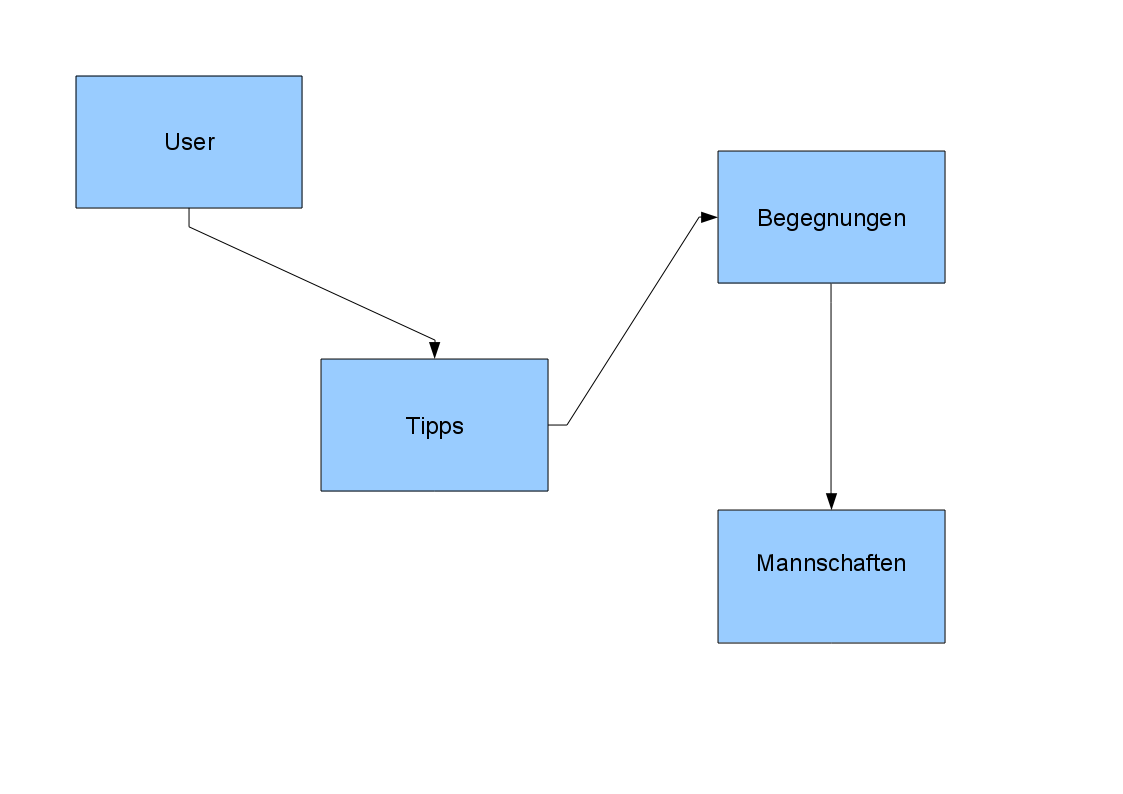
\includegraphics[scale=0.5]{pictures/klassen.png}
 \end{center}
 \caption{Benötigte Klassen}
 \label{klassen}
\end{figure}

Im Zentrum stehen die Tipps, welche die User abgeben können. Die Tipps setzen
sich zusammen aus den einzelnen Usern (Tipper) und den Spielbegegnungen. In
diesem Fall die Spiele der WM 2010. Weiterhin setzen sich diese aus Den
Mannschaften und weiteren Informationen, wie Spielzeit den Ergebnissen zusammen.
\\
\\

\begin{lstlisting}[caption=Modelle in Django]{Name}
class Tipps(models.Model):
    user = models.ForeignKey(User, unique=False)
    begegnung = models.ForeignKey(Begegnung, unique=False)
    
    toreHeim = models.IntegerField(max_length=2)
    toreGast = models.IntegerField(max_length=2)
    tippDatum = models.DateTimeField()
    
    def __unicode__(self):
        return u'%s %s' % (self.user, self.begegnung)
   
\end{lstlisting}

Mit Hilfe des eingebauten OR-Mappers in Django können die Tabellen aus den
vorher definierten Klassen als Tabellen in die Datenbank gespeichert werden.
Die Speicherung bzw. Synchronisation geschieht mit Django eigenen Boardmitteln.

\begin{lstlisting}[caption=Datenbanksynchronisation]{sync}
python manage.py syncdb
\end{lstlisting}

Damit python mit der Datenbank kommunizieren kann muss vorher ein
Datenbank-Connector installiert werden. Django unterstützt Oracle, PostgreSQL,
MySQL und SQLite. Die Installation des Connectors ist abhängig von der
Datenbank, die benutzt werden soll. Getestet wurden mySQL und PostgreSQL
hierbei bei der lokalen Entwicklung unter Ubuntu mySQL und auf den
Applikationsserver Postgres.

\section{Views}
\section{Registrierung}
\section{Hilfsskripte}
\section{Templates}
\section{Portierung auf Produktionsserver}
\section{Fazit}


\end{document}
